\chapter{Conclusion}
\label{chap:90conclusion}

\noindent
Finally, we conclude the thesis by summarizing its results
and by giving an outlook on possible future work.
In particular, we highlight key contributions of the thesis to research,
give recommendations for future applications of the presented method, and
state possible downsides and limitations.

\vspace*{-0.5em}

\paragraph{Summary of the thesis}

The contribution of this thesis consisted of two major parts.
In the first part,
hierarchical B-splines on sparse grids were comprehensively presented
and embedded in a sparse grid framework with general
tensor product basis functions.
The advantage of this approach was that the framework could be reused
for different hierarchical bases
(as for the various spline bases derived in this thesis)
and that it clarified which properties only held for the
classical piecewise linear bases and not for other tensor product bases.
We saw that standard hierarchical B-splines suffer from
approximation issues near the boundary, and
we resolved these issues by incorporating not-a-knot boundary conditions
into the hierarchical B-spline basis.
In the further course of the thesis,
the focus was put on the algorithmic implications of the novel bases,
taking the hierarchization problem as an example.
We looked at requirements that had to be satisfied by grids and bases
to enable efficient hierarchization algorithms
such as breadth-first search and unidirectional principle,
for which we gave clear formulations and formal correctness proofs.
As a result, a whole ``zoo'' of hierarchical (B-)spline functions
has been derived in this thesis.
The main types were
standard hierarchical B-splines,
modified hierarchical B-splines,
hierarchical not-a-knot B-splines,
hierarchical fundamental splines, and
hierarchical weakly fundamental splines
(where the first two are not novel).
Modified, not-a-knot, and (weakly) fundamental splines could be combined
almost arbitrarily to tailor the ansatz functions to suit one's specific needs.

\pagebreak

The second, more practical part of the thesis was dedicated to transferring
the newly gained theoretical knowledge to
academic and real-life application test cases.
We verified that only with the new hierarchical not-a-knot conditions,
one is able to obtain the best possible order of convergence
$\landauO{\ms{n}^{p+1}}$ for interpolation
(B-spline degree $p$, fixed dimensionality $d$).
Using the Novak--Ritter criterion,
which was specifically designed for optimization,
we were able to achieve optimization gaps
that were for some test functions up to six orders of magnitude smaller
for cubic B-splines than for standard piecewise linear functions.
We transferred the Novak--Ritter criterion to uncertainty quantification
and obtained similarly strong results for the
propagation of fuzzy uncertainties with the fuzzy extension principle.
Furthermore, we successfully showed the suitability of hierarchical B-splines
for three real-world applications,
which are summarized in \cref{tbl:applicationSummary}.
\begin{table}
  \setnumberoftableheaderrows{1}%
  \begin{tabular}{%
    >{\kern\tabcolsep}=l<{\kern5mm}+l+l+l<{\kern\tabcolsep}%
  }
    \toprulec
    \headerrow
    Category&                   Topology opt.&      Biomechanics&      Finance\\
    \midrulec
    Interpolated quantities&    Elasticity tensors& Muscle forces&     Value functions\\
    SG dimensionality&          5&                  2&                 5\\
    \#Optimization variables&   \num{40000}&        2&                 11\\
    Time per evaluation&        \SI{30}{\second}&   \SI{30}{\minute}&  ---\\
    \#Eval. per opt. iteration& \num{8000}&         4&                 150\\
    Objective function type&    Non-linear&         Linear/non-linear& Non-linear\\
    Constraint function type&   Non-linear&         Non-linear/---&    Linear\\
    Optimization method&        SQP&                Augm. Lagrangian&  SQP\\
    \bottomrulec
  \end{tabular}
  \caption[%
    Summary of characteristics of the applications%
  ]{%
    Summary of characteristics of the applications presented in this thesis.
    The given values are rough example values that
    represent possible application test cases.%
  }%
  \label{tbl:applicationSummary}%
\end{table}%
First, by interpolating Cholesky factors of elasticity tensors,
we accomplished to efficiently solve
topology optimization problems in three spatial dimensions
with complex micro-cell structures.
Second, in the biomechanical application,
we dramatically reduced the computational time to solve
test scenarios by up to \SI{99}{\percent} by using
sparse grid surrogates with B-splines instead of the
exact continuum-mechanical model.
Third, we were able to solve dynamic portfolio choice problems
with five state variables and eleven policy variables
with unprecedented precision, as one could only speculate
how the solution looked like with state-of-the-art methods.
In all of these applications, the advantages of B-splines were made clear
by comparing the results to the classical piecewise linear basis.
The implementation of hierarchical B-splines of sparse grids is
publicly available as part of the sparse grid toolbox \sgpp
under a free and open-source license.%
\footnote{%
  \url{http://sgpp.sparsegrids.org/}%
}

\vspace*{\fill}
\pagebreak

\paragraph{Recommendations (advantages and disadvantages)}

Despite its broad applicability,
the presented method of B-splines on sparse grids is of course
not suited for all possible scenarios.
One must be able to sample the objective function at arbitrary
locations in some hyper-rectangle in order to use sparse grids;
a prescribed point cloud of scattered data does not suffice.
Moreover, the problem should not have more than ten dimensions,
since convergence notably slows down as the dimensionality grows,
although spatially adaptive approaches might still be feasible for
higher dimensionalities \cite{Pflueger10Spatially}.
In addition, the objective function should be ``as smooth as possible''
in order to benefit from higher-order B-splines.
This means ``continuous'' at the very least,
but twice continuous differentiability is more desirable.
The general rule is that the objective function should be
at least as smooth as the employed basis functions in order to obtain
optimal convergence results.
The concrete choice of basis (general type and degree) depends
on the application:
Not-a-knot B-splines are well-suited for objective functions with
dominating near-polynomial parts.
Fundamental splines may be used to accelerate the process of
hierarchization by enabling breadth-first search in quadratic time.
With weakly fundamental splines, this can be further reduced to
linear time using the unidirectional principle.
However, the additional grid points that have to be inserted
have to be taken into account as well.
The rule of thumb is that the more spatially adaptive a sparse grid is
(i.e., only few high-level grid points),
the more points have to be inserted.
In general, it does not hurt to try the different available
B-spline types and degrees,
since most function values can simply be reused
once the objective function has been sampled.

\vspace*{\fill}

\paragraph{Outlook and future work}

Finally, we briefly give suggestions for possible future work.
A major topic of interest is that of refinement criteria and adaptivity.
Besides the Novak--Ritter criterion,
there are other refinement criteria that are tailored to optimization
such as simultaneous optimistic optimization \cite{Wang14Bayesian}.
In addition, nested methods for hierarchical optimization could
use multiple interpolants with different resolutions
on different grids \cite{Delbos14Global}.
Criteria that directly incorporate constraints would improve
results in constrained optimization settings.
With respect to adaptivity,
there is also much work left to do.
This thesis focused on spatial adaptivity for its applications,
but there are interesting applications
that greatly benefit from dimensional adaptivity,
for example plasma physics \cite{Pflueger14EXAHD}.
Another key task would be the introduction of
$h$-$p$-adaptivity to B-splines on sparse grids,
which would greatly enhance the applicability of B-splines in
non-smooth scenarios.
As a simple special case,
one could investigate different B-spline degrees in different dimensions.
However, true $h$-$p$-adaptivity would allow to locally choose
both the spatial resolution $h$ and the B-spline degree $p$,
adapting them according to the local smoothness of the function.

\pagebreak

With regard to the application side, there are also quite a few
possibilities for future work.
The sparse grids in the biomechanical application
we considered in this thesis were only two-dimensional.
This is not in the range of dimensions in which sparse grids
demonstrate their full strength,
although the two-dimensional surrogates were already able to drastically
reduce the required computation time compared to full grids.
Currently, an extended model with five muscles and therefore
five-dimensional sparse grids is being considered
(see \cref{fig:upperLimb5D}).
\begin{SCfigure}
  \begin{tikzpicture}
    \node[anchor=south west] at (0mm,0mm) {%
      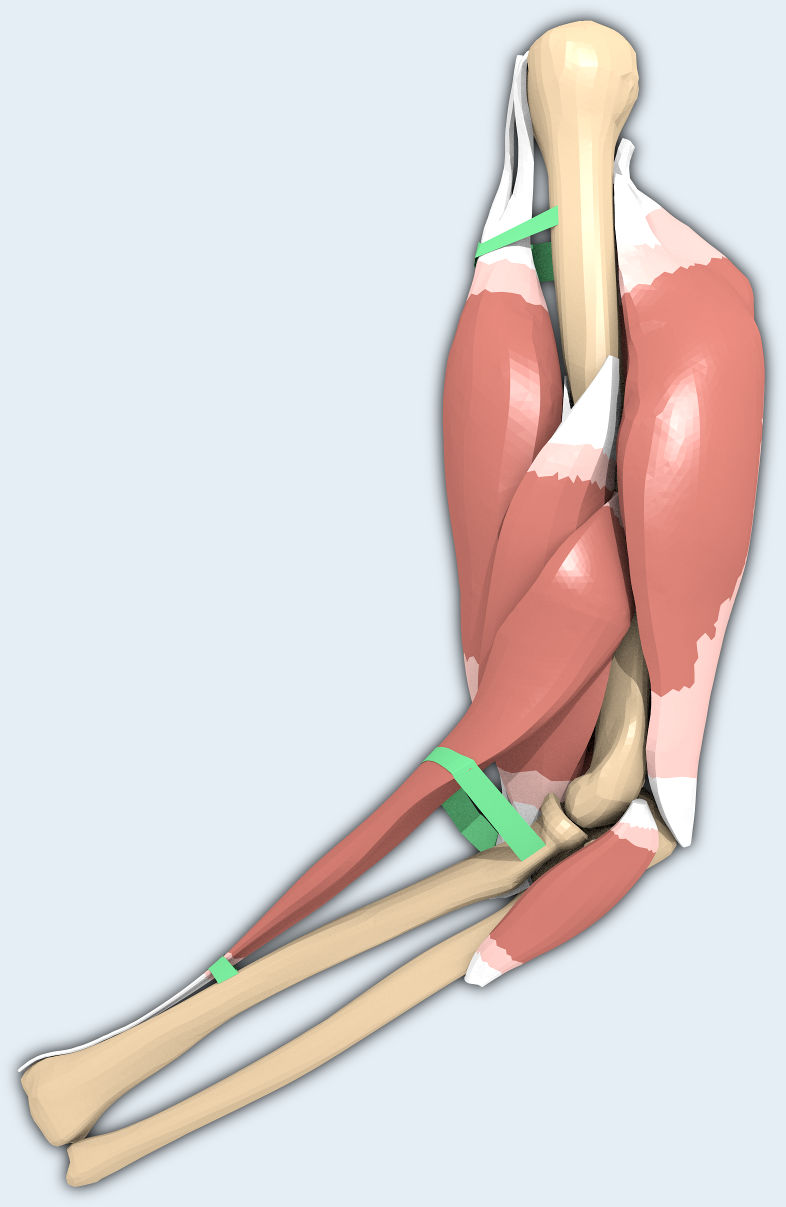
\includegraphics[height=80mm]{upperLimb5D}%
    };
    \node[anchor=west] (humerus)    at (0mm,75mm)  {\small{}Humerus};
    \node[anchor=west] (radius)     at (0mm,20mm)  {\small{}Radius};
    \node[anchor=east] (ulna)       at (40mm,10mm) {\small{}Ulna};
    \node[anchor=east] (triceps)    at (73mm,52mm) {\small{}Triceps};
    \node[anchor=west] (biceps)     at (0mm,52mm)  {\small{}Biceps};
    \node[anchor=west] (brachialis) at (0mm,44mm)  {\small{}Brachialis};
    \node[anchor=west] (brachioradialis) at (0mm,36mm) {%
      \small{}Brachioradialis%
    };
    \node[anchor=east] (anonceus)   at (73mm,20mm) {\small{}Anonceus};
    \draw (humerus)         -- (39mm,75mm);
    \draw (radius)          -- ($(0mm,10mm)!(radius)!(20mm,10mm)$);
    \draw (ulna)            -- (20mm,10mm);
    \draw (triceps)         -- (48mm,52mm);
    \draw (biceps)          -- (33mm,52mm);
    \draw (brachialis)      -- (36mm,44mm);
    \draw (brachioradialis) -- (36mm,36mm);
    \draw (anonceus)        -- (38mm,20mm);
  \end{tikzpicture}%
  \caption[Extended model of the human upper limb with five muscles]{%
    Extended model of the human upper limb with
    the three bones humerus, radius, and ulna
    \emph{\textcolor[RGB]{191,162,118}{(light brown)}} and
    the five muscles
    triceps, biceps, brachialis, brachioradialis, and anonceus
    \emph{\textcolor[RGB]{150,58,46}{(red)}.}
    Each muscle has associated tendon
    \emph{\textcolor[RGB]{128,128,128}{(white)}}
    and muscle-tendon complexes
    \emph{\textcolor[RGB]{255,160,160}{(light red)}.}
    Biceps and brachioradialis have each been fixed with one and two bands
    \emph{\textcolor[RGB]{80,200,100}{(green)}}
    to simulate the effect of the missing skin.
    Without bands, the muscles would unnaturally raise from the bones.%
  }%
  \label{fig:upperLimb5D}%
\end{SCfigure}%
Here, it will be mandatory to employ spatial adaptivity
to cope with the increased dimensionality.
In the application of topology optimization,
more complicated micro-cell models and more complicated
settings could be studied.
For example, the widths of the diagonal macro-bars could be constrained
\cite{Allaire16Towards}.
The dynamic portfolio choice models in the financial application
were quite limited.
For example,
there was no inheritance motive (i.e., bequest),
the model did not contain the individual's regular income, and
the model did not account for savings for large necessary investments
(e.g., cars or houses), which seems unnecessarily unrealistic.
Finally, one could consider many other real-world optimization problems
or other application fields of B-splines on sparse grids,
for instance, data mining or uncertainty quantification.
If objective gradients are available besides function values,
it might be feasible to directly incorporate the gradients into
the interpolation scheme \cite{Baar15Gradient}.

This extensive but by no means exhaustive list of possible future work
can be seen as an inspiration and starting point
for new and interesting applications of B-splines for sparse grids.

\cleardoublepage
